\section{Solid Isotropic Material with Penalization (SIMP)}

\subsection*{Volume-to-Point (VP) Heat Conduction Problem}

Consider a finite-size volume in which heat is being generated at \textit{every} point, and which is cooled through a small patch (the heat sink) located on its boundary. Suppose that we have a finite amount of high-conductivity ($k_+$) material available. Our goal is to determine the optimal distribution of the $k_+$ material through the given volume such that \textit{the highest temperature is minimized}.

Solid Isotropic Material with Penalization (SIMP) is a method based on topology optimization that can be used to solve the VP Heat Conduction Problem. SIMP is what is called a soft kill method, meaning that in each step of the method we increase or decrease high-conductivity material by a small quantity. This allows us to apply methods designed for continuous optimization problems to this discrete problem.

\subsection{SIMP Method Description}

\subsubsection*{Assumptions}
In order to develop the method, we need to make a couple of assumptions.

First of all, the energy differential equation driving the heat-flux inside the finite-volume requires:
\begin{enumerate}
	\item All calculations are run under steady-state conditions. That is, all heat produced in the volume is evacuated through the heat sink.
	\item Low-conductivity materials ($k_0$) and high-conductivity materials ($k_+$) are treated as homogeneous and isotropic on their respective conductivities.
\end{enumerate}

Throughout the article \cite[]{Marck2012}, the authors also set the following conditions:
\begin{itemize}
	\item Thermal conductivities are constant:
	$$k_0=1 \si[per-mode=fraction]{\watt\per\square\meter\per\kelvin}\qquad\text{and}\qquad k_+=100 \si[per-mode=fraction]{\watt\per\square\meter\per\kelvin}$$
	\item All structures have a square aspect ratio with $L=H=0.1\si{\meter}$
	\item The heat-sink is located on the middle of the west side of the structure
	\item The heat-sink has Dirichlet boundary conditions: $T_S=0\si{\celsius}$
	\item All other boundaries are adiabatic: $\nabla T=0$
\end{itemize}

\subsubsection*{Notation}

We have the following sets to describe the VP-problem:
\begin{itemize}
	\item $\vec{x}\in\Omega$ = two-dimensional spatial field
	\item[] We set $\Omega = \Omega_0\cup\Omega_+$ where
	\begin{itemize}
		\item $\Omega_0$ = portion of $\Omega$ that has conductivity $k_0$. This is the portion of the space where we have not placed any high-conductivity material.
		\item $\Omega_+$ = portion of $\Omega$ with conductivity $k_+$. This is the portion of the space with the high-conductivity material applied.
	\end{itemize}
	\item $\vec{k}\in\mathbb{K}$ = distribution of high-conductivity material
	\item $T\in\overline{\mathbb{T}}$ = temperature field that satisfies the energy equation $\nabla\cdot\left(\vec{k}\nabla T_{\vec{k}}\right)+q=0$ where $q$ is the local heat-generating rate.
\end{itemize}

\subsection{The Optimization Problem}

Using the above established notation, we develop the following optimization problem:

	\begin{equation}
		\begin{tabular}{lll}
			\text{minimize }   & $f(T)$ & \text{for } $T\in\mathbb{T},\vec{k}$      \\
			\text{subject to } & $\nabla\cdot\left(\vec{k}\nabla T_{\vec{k}}\right)+q=0$ & \\
			& $\vec{x}\in\Omega,\quad\vec{k}\in\mathbb{K}_{\text{ad}}$&      
		\end{tabular}\label{SIMP-Optimization-Problem}
	\end{equation}

\subsubsection*{Penalization Process}
The problem of whether to place high conductivity material in a particular location or not is discrete in nature. This is unfortunate as continuous optimization problems are generally easier to solve. In particular, we cannot apply some of the optimization methods described earlier, such as gradient descent, to a discrete optimization problem as they require the optimization variables to be continuous.

The SIMP method has a clever way of getting around this particular issue of discrete variables: create a continuous function that allows for a ``mix'' of the two conductive materials. This function turns our discrete variables into a continuous one, allowing us to apply the nice methods used in continuous optimization problems. However, in reality, we cannot actually mix the two conductive materials and therefore need a solution that produces a 1---0 structure. That is, our final result needs to either have conductivity $k_0$ or $k_+$ at each point, not some fraction of each. Therefore, in each iteration of the SIMP process, we \textit{penalize} the mixing of the material. Keeping this in mind we introduce a design parameter $\eta\in\left[0,1\right]$ that controls the amount of mixing of the two materials:
\begin{equation}
	k\left(\eta\right)=k_0+\left(k_+-k_0\right)\eta^p\qquad\text{with}\qquad 0\leq\eta\leq 1\qquad\text{and}\qquad p\geq1.\label{eqn:penalization}
\end{equation}
An added bonus of this formulation of $k(\eta)$ is that it is of the form \eqref{eqn:Convexity}, and hence a convex function! Notice that when $\eta=0$, $k\left(0\right)=k_0$ and when $\eta=1$, $k\left(1\right)=k_+$. The value $p$ in \eqref{eqn:penalization} is the \textit{penalization parameter}. $p$ aids in the convergence process; without $p$ the SIMP method converges to a structure that is not 1---0: a composite structure where finite-volumes are made up of different proportions of $k_0$ and $k_+$ materials.

To converge to a 1---0 structure, we gradually increase $p$ beginning from $p=1$. Increasing $p$ from $1$ puts the objective function in \eqref{SIMP-Optimization-Problem} at a disadvantage if $\eta\neq1$. Once $p$ gets much larger than $1$ the second term in $k(\eta)$ of \eqref{eqn:penalization} becomes much smaller than $k_0$ and hence $k(\eta)\approx k_0$ for values of $\eta\neq1$. As a result, when trying to optimize $f(T)$, value of $\eta$ in $(0,1)$ are penalized which leads to design parameters taking on values of $0$ or $1$, creating a 1---0 structure.

\subsubsection*{``King Me'': Avoiding the Checkerboard Problem}

If one were to optimize conductive material placement to increase heat transfer on a standard rectangular grid, a simplistic solution would be to create a grid of alternating material types in each adjacent rectangle, like a checkerboard. This way, the heat is always flowing to adjacent cells. While this may indeed increase heat transfer, it doesn't necessarily decrease the average temperature in our object (or transfer the heat towards the heat-sink). Hence, avoiding this non-physical checkerboard solution is of concern.

\begin{figure}
	\centering
	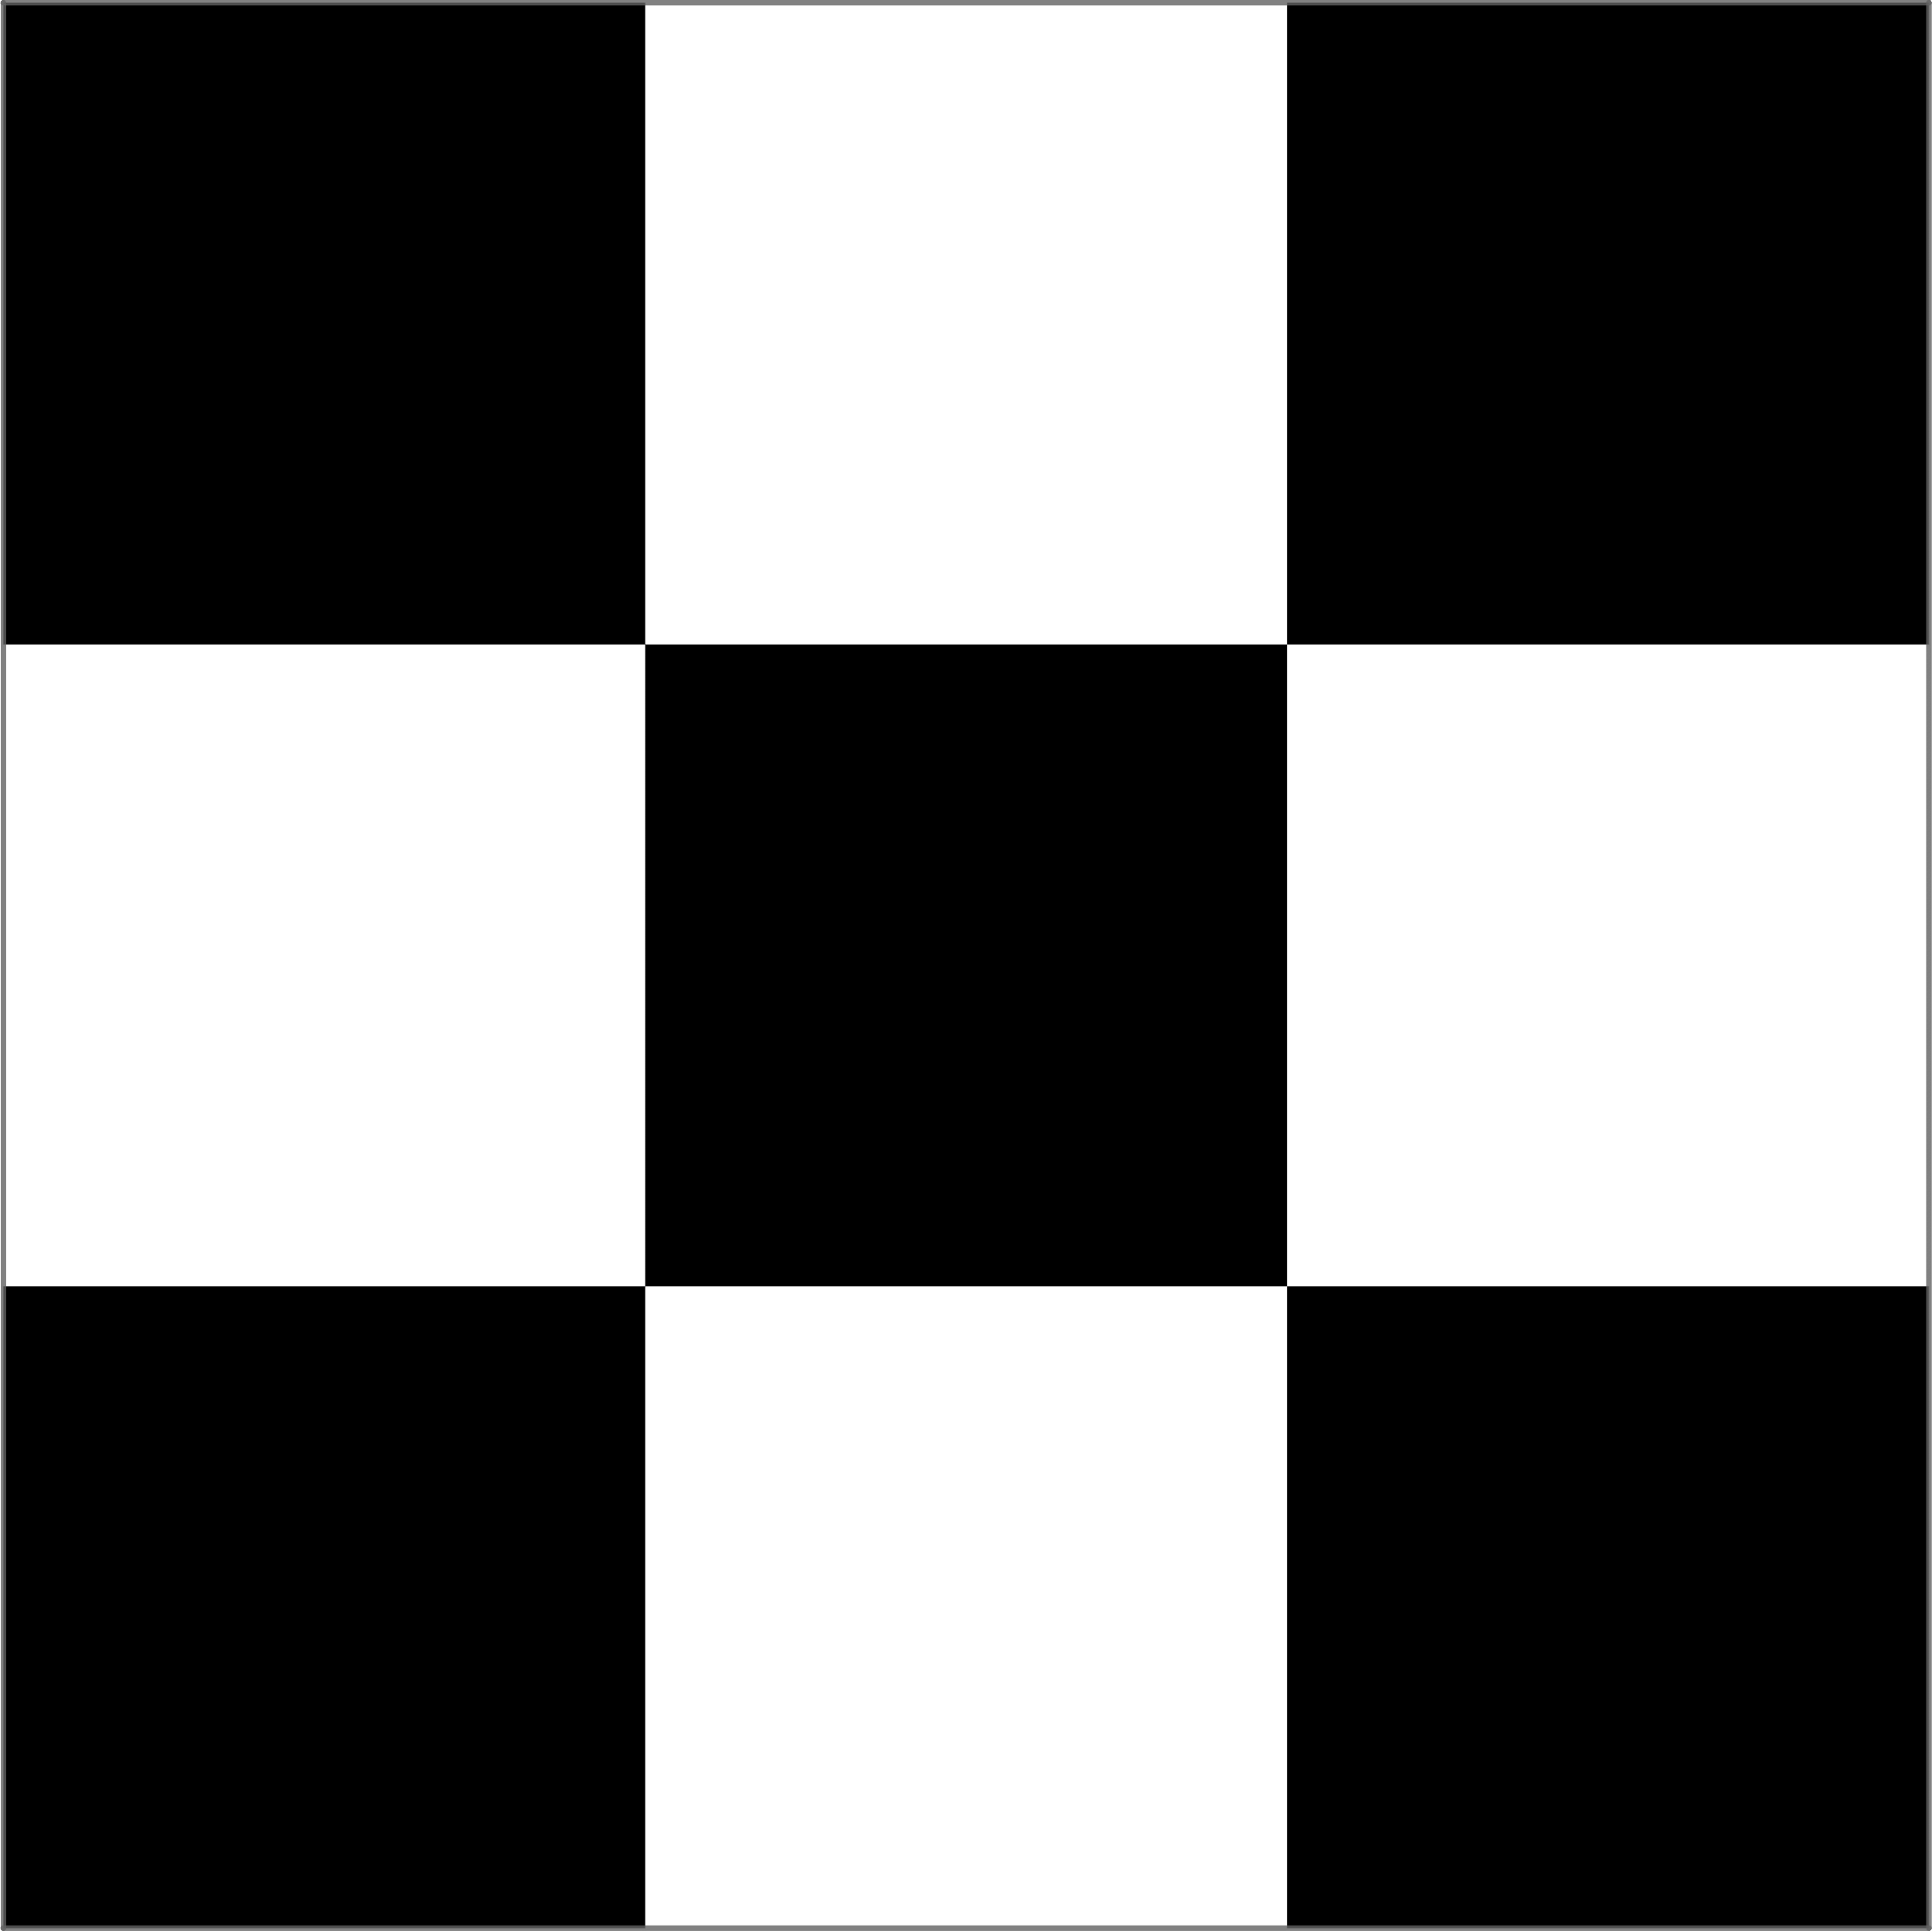
\includegraphics[width=0.4\textwidth]{Chapter_II_SIMP_Optimization/Images/3x3-Checkerboard.png}
	\caption[Checkerboard Pattern]{A checkerboard pattern result on a 3-by-3 control volume grid. The black spaces represent areas where $\eta=1$ and the white spaces represent areas where $\eta=0$ in \eqref{eqn:penalization}. This results in adjacent regions of alternating thermal conductivites $k_+$ and $k_0$, artificially maximizing heat transfer between control volumes.}
	\label{fig:3x3-Checkerboard}
\end{figure}

\begin{figure}
	\centering
	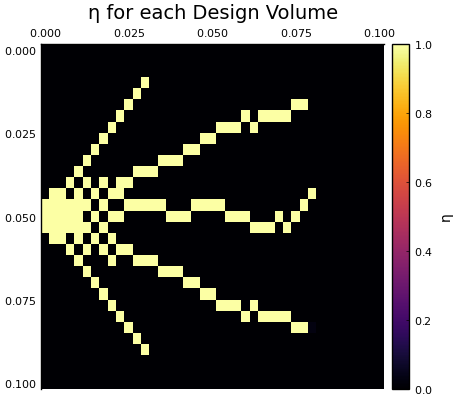
\includegraphics[width=0.6\textwidth]{Chapter_II_SIMP_Optimization/Images/SIMP-Example-Checkerboarding.png}
	\caption[Checkerboard Result in Practice]{Output of SIMP algorithm for $30\times 40$ temperature control volumes. Notice the local checkerboarding around $(0.05,0.015)$.}
	\label{fig:SIMP-Checkerboard}
\end{figure}

In order to solve the heat equation \eqref{eqn:HeatEq}, we employ the Finite Volume Method (described earlier). This involves splitting up our space into a finite number of control volumes. The checkerboard pattern emerges when the solution of our optimization process converges to a 1---0 structure which has some meshes that successively belong to the $\Omega_0$ and $\Omega_+$ sets (i.e.: adjacent grid volumes have alternating thermal conductivites). As a result, the heat transfer within the structure between $k_+$ and $k_0$ regions is maximized, artificially increasing the impact of adding $k_+$ material on the temperature $T$, which in turn minimizes the objective function in \eqref{SIMP-Optimization-Problem} \cite[]{Versteeg2007}. Typically, this pattern occurs locally but then spreads throughout the entire structure through successive iterations of the optimization process. However, in the real world, these checkerboard placements of our conductive materials do not actually have the effect of lowering the average temperature in structures. In fact, the checkerboard example in Figure \ref{fig:3x3-Checkerboard} doesn't even direct heat towards the heat-sink on the left wall of the structure.

In order to avoid obtaining checkerboard solutions from our optimization process, we employ two separate staggered grids for our temperature and design variables. We need to employ some extra equations in order to translate between design and temperature variables, but this strategy adequately solves the issue of convergence to checkerboard solutions.

\begin{figure}
	\centering
	\ctikzfig{Chapter_II_SIMP_Optimization/Images/Grid}
	\caption[Overlayed Design \& Temperature Grids]{Overlayed Temperature (\rule[0.55ex]{1.25em}{1.5pt}) and Design (\rule[0.6ex]{0.4em}{0.5pt}\,\rule[0.6ex]{0.4em}{0.5pt}\,\rule[0.6ex]{0.4em}{0.5pt}) grids with $4\times4$ Design Element $(\eta^{i,j})$ and $3\times3$ Temperature Control Volume $(K_C^{i,j})$ Nodes. $K_N^{i,j}$ and $K_W^{i,j}$ indicate nodes at the North and West boundaries, respectively, of each Temperature Control Volume. Each Temperature control volume is numbered beginning in the upper left and continuing column-by-column, left-to-right.}
	\label{fig:grids}
\end{figure}

One of the grids contains the information related to the temperature scalars and the other stores information related to the design parameters, $\eta$.

\subsection{Finite Volume Method Discretization}

Any discretization method could be used to numerically solve the heat equation \eqref{eqn:HeatEq}. In our implementation of the SIMP algorithm, the Finite Volume Method (described earlier in \S\ref{sec:FVM}) was used. FVM is used to discretize the formation of the heat equation in \eqref{SIMP-Optimization-Problem}:
\begin{equation}
	\nabla\cdot\left(k\nabla T\right)+q=0\label{eqn:SIMP-Heat-Eq}.
\end{equation}
We create a rectangular grid of $N_T=m\times n$ temperature control volumes of size $\Delta x\times\Delta y$ (solid squares in Figure \ref{fig:grids}). Each element is indexed by $1\leq i\leq m$ and $1\leq j\leq n$, where $i$ refers to the row and $j$ the column of the control volume. The volume indexed $(i,j)=(1,1)$ is located in the upper-left and $(i,j)=(m,n)$ in the bottom-right corner of the object. The temperature over the area of the temperature control volume $(i,j)$ is considered to be $T^{i,j}$.

Around the upper left corner of each temperature control volume we create a corresponding design element (dashed squares in Figure \ref{fig:grids}). The area within each $(i,j)$ design element has conductivity $k^{i,j}=k(\eta^{i,j})$ as evaluated by \eqref{eqn:penalization}.

In order to employ the finite volume method, it is necessary to be able to calculate the temperature fluxes along the boundaries of each control volume. To do this, we need to have a value for the conductivity along the faces of each control volume. Notice that the faces of the temperature control volumes lie within two adjacent design regions, which implies that there are two different conductivites along that face. To create a consistent conductivity along the control volume wall, we average (using either an arithmetic or harmonic mean) the conductivity of the two adjacent design nodes. Hence the conductivity along the West face of control volume $(i,j)$, denoted by $k^{i,j}_W$, is given by
\begin{equation}
	\text{Arithmetic Mean: }k^{i,j}_W=\frac{k^{i,j}+k^{i+1,j}}{2}\qquad\text{or}\qquad\text{Harmonic Mean: }k^{i,j}_W=2\left(\frac{1}{k^{i,j}}+\frac{1}{k^{i+1,j}}\right)^{-1}.\label{eqn:k_W-Average-Filter}
\end{equation}
Similarly, the conductivity along the North face of control volume $(i,j)$, denoted by $k^{i,j}_N$, is given by
\begin{equation}
	\text{Arithmetic Mean: }k^{i,j}_N=\frac{k^{i,j}+k^{i,j+1}}{2}\qquad\text{or}\qquad\text{Harmonic Mean: }k^{i,j}_N=2\left(\frac{1}{k^{i,j}}+\frac{1}{k^{i,j+1}}\right)^{-1}.\label{eqn:k_N-Average-Filter}
\end{equation}

For temperature control volume $(i,j)$, the finite volume method discretizes \eqref{eqn:SIMP-Heat-Eq} into the following linear equation
\begin{equation}
	K^{i,j}_C T^{i,j}=K_W^{i,j}T^{i,j-1}+K_W^{i,j+1}T^{i,j+1}+K_N^{i,j}T^{i-1,j}+K_N^{i+1,j}T^{i+1,j}+Q^{i,j},\label{eqn:FVM-Discret}
\end{equation}
where the $K^{i.j}$ terms represent the diffusive flux coefficients, $T^{i,j}$ the temperature of control volume $(i,j)$, and $Q^{i,j}$ the heat generation of volume $(i,j)$.

The value of the flux at the center node of the control volume is equal to the total flux through the volume faces, so we have an additional equation to pair with \eqref{eqn:FVM-Discret}:
\begin{equation}
	K^{i,j}_C=K_W^{i,j}+K_W^{i,j+1}+K_N^{i,j}+K_N^{i+1,j}\label{eqn:CenterFluxCoeff}
\end{equation}

The $K_W$ and $K_N$ coefficients are dependent on the thermal conductivity and cross-sectional area of their corresponding faces:
\begin{equation}
	K_W^{i,j}=\frac{k_W^{i,j}\Delta y}{\Delta x}\qquad\text{and}\qquad K_N^{i,j}=\frac{k_N^{i,j}\Delta x}{\Delta y}\label{eqn:K-Coeffs}
\end{equation}

Putting together \eqref{eqn:k_W-Average-Filter}, \eqref{eqn:k_N-Average-Filter}, \eqref{eqn:FVM-Discret}, \eqref{eqn:CenterFluxCoeff}, and \eqref{eqn:K-Coeffs} for all $N_T$ control volumes gives us a system of equations that discretize \eqref{eqn:SIMP-Heat-Eq}. Collecting the coefficients $K$ into a matrix and representing the $T$ and $Q$ values as vectors, and doing a little reorganizing, we can represent the system of equations as a matrix equation:
\begin{equation}
	\mathbf{K}\mathbf{T}=\mathbf{Q}.
\end{equation}

Let us take a moment to analyze the structure of the matrix $\mathbf{K}$, as it might not be immediately evident to the reader what the elements of this matrix represent. (It took the author some time to interpret the meaning of this matrix.) $\mathbf{K}$ is a sparse, symmetric, and pentadiagonal $mn\times mn$ matrix.

The entries in the matrix $\mathbf{K}$ indicate the coefficient of diffusive flux between numbered temperature control volumes. Notice in Figure \ref{fig:grids} how the temperature control volumes are numbered down the columns. Entry $\mathbf{K}[\alpha,\beta]$ is the flux coefficient between volumes number $\alpha$ and $\beta$. Since the flux coefficient between volumes $\alpha$ and $\beta$ is the same as that between $\beta$ and $\alpha$, $\mathbf{K}[\alpha,\beta]=\mathbf{K}[\beta,\alpha]$, producing the symmetry of matrix $\mathbf{K}$.